\section{Arquitectura y diseño del sistema}

\subsection{Sistema monolítico frente a basado en microservicios}

Durante los últimos años, en parte gracias a la aparición de plataformas cloud como AWS, Azure o Google Cloud, se ha popularizado el desarrollo de sistemas basados en microservicios, que conectados entre ellos mediante diversos protocolos de comunicación, forman un sistema completo. Debido a esto, para el desarrollo del código necesario referente al servidor, consideré tanto desarrollar un sistema basado en microservicios como un sistema de código monolítico.

En primer lugar, analicé las ventajas e inconvenientes que me podía ofrecer un sistema basado en microservicios. Una de las principales ventajas que se les atribuye a estos sistemas es ``la facilidad para escalar el sistema en comparación con un sistema monolítico'' \cite{arquitectura-comp1}. Durante los años los colaboradores de la fundación no han sido tan numerosos como para necesitar un sistema que soporte a miles de usuarios. En este caso, debido a que el número de usuarios del sistema será pequeño y constante, esto no será un problema \cite[p.~4]{monolith1}.

Por otra parte, son más convenientes para un desarrollo en equipo. Cuando cada parte de un equipo de desarrollo se dedica a una funcionalidad, facilita mucho que estas estén separadas en servicios independientes. Esto tampoco sería una ventaja en este caso, debido a que el equipo de desarrollo consta de una sola persona. 

Una de las desventajas a la hora de utilizar microservicios en esta situación sería la de la gestión del alojamiento. Para alguien con un conocimiento informático bajo, será más fácil gestionar un sistema al completo, antes que gestionar cada uno de los servicios, lo que conllevaría un conocimiento de como funciona cada uno de estos y como se comunican entre ellos.

Al no ser un sistema complejo un sistema monolítico casa perfectamente con lo que se busca. Proporcionará un desarrollo menos complejo, a la hora de solo tener que desarrollar y comprender una base de código. Además, una más fácil integración y despliegue con los servicios de alojamiento, así como una más fácil comprensión y depuración del sistema, hace que los sistemas monolíticos sean la elección correcta para este caso.

\subsection{Arquitectura del sistema}
\label{sec:arq}

A la hora de desarrollar el sistema se consideró utilizar una arquitectura basada en el paradigma Modelo, Vista, Controlador \cite{mvc}, mostrada en la Figura \ref{fig:arq}. 

\begin{figure}[H]
    \centering
    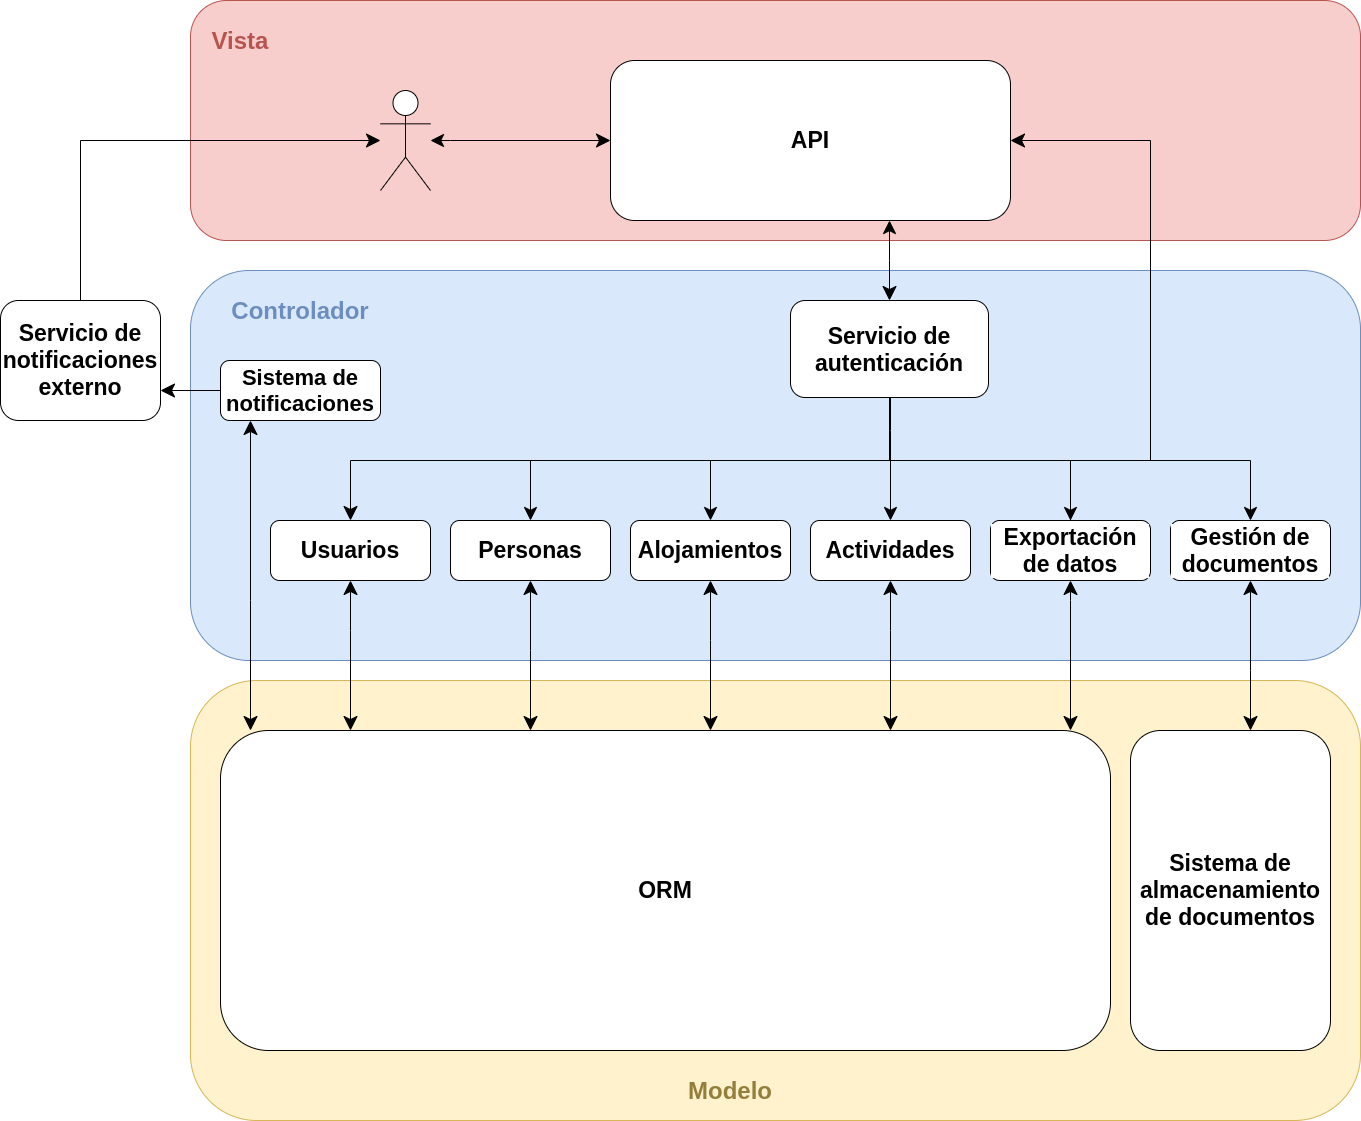
\includegraphics[width=\textwidth]{diseno/sistema/Arquitectura.png}
    \caption{Arquitectura del sistema}
    \label{fig:arq}
\end{figure}

Dentro de la \textit{vista} se ha incluido tanto la parte de la aplicación desarrollada en este proyecto como futuras implementaciones de webs u otras interfaces que se conecten con el sistema, representado con el usuario. Aquí dentro he considerado incluir también la API en representación a las rutas de esta, que guían a los servicios del controlador correspondientes según cada una. 

En el \textit{Controlador}, cualquier llamada a la API pasará por el \textit{Servicio de autenticación}, que se encargará de garantizar que ningún usuario del sistema acceda a un recurso o servicio no permitido. Una vez este de acceso a los recursos del sistema se llamará a cualquiera de los módulos comprendidos en el sistema. Estos albergan la lógica de negocio necesaria en cada uno de los casos y proporcionarán directamente la salida correspondiente a la vista. Entre estos módulos se destacan los que se encargan de realizar operaciones CRUD (Create, Read, Update and Delete) en el modelo (\textit{Usuarios},\textit{Personas},\textit{Alojamientos},\textit{Actividades}). Además de estos, se encuentran los módulos \textit{Sistema de notificaciones}, \textit{Exportación de datos} y \textit{Gestión de documentos}, los cuales realizar tareas más específicas.

En cuando al \textit{Modelo}, el \textit{ORM} correspondiente se encargará de acceder y modificar datos en la base de datos y el \textit{Sistema de almacenamiento de documentos}, de hacer lo mismo con documentos y fotografías.   

\subsection{Diseño de la base de datos}

Al elegir utilizar bases de datos relacionales, uno de los primeros pasos era el diseño. Para este se realizó el diagrama E/R correspondiente (Figura \ref{fig:er}) centrando el diseño en la parte principal, las personas. Para estas se diseño una tabla con los atributos compartidos entre los diferentes tipos, a la cual se añadió una herencia para cada uno de ellos. Algunos atributos de las personas, los cuales necesitaban de multiplicidad, se han añadido como tablas a parte, como es el caso entre otras de las tablas \textit{nacionalidad} o \textit{colectivo}. Por otra parte, las altas y bajas se gestionarán mediante una tabla, para la cual se tendrá que comprobar que la información introducida es coherente, es decir, que cuando alguien está de alta, no se pueda introducir un alta de nuevo, o que no se puedan introducir bajas cuando no existe un alta. Por último, se contempla que las personas tengan relaciones entre ellas. Esto se hace mediante la tabla \textit{relación}, la cual contempla el tipo de relación (madre, padre, hijo, tío, sobrino...).

Con respecto a los documentos y fotografías, se ha creado una tabla que almacena la ruta del archivo en el sistema de almacenamiento de archivos permitiendo que mediante una llamada a la ruta correspondiente de la API, se pueda recuperar este.

La parte de alojamiento de la aplicación está reflejada en las tablas \textit{Habitación} y \textit{Casa}. La habitación estará formada por varios residentes y un residente solo podrá pertenecer a una habitación, formando una relación \textit{1:N}. Entre casas y habitaciones ocurre el mismo tipo de relación. 

El apartado de actividades del sistema estará reflejado mediante la tabla \textit{Actividad} a la cual se relacionarán los residentes cuando un usuario con un residente asociado se apunta a la actividad. La tabla \textit{Ranking} será una tabla calculada en base a las tablas \textit{actividad} y \textit{participación}, que permitirá que aun generando duplicidad de los datos, la recuperación de estos a la hora de obtener las puntuaciones de todos los usuarios se realice en un tiempo aceptable. 

\begin{figure}[]
    \centering
    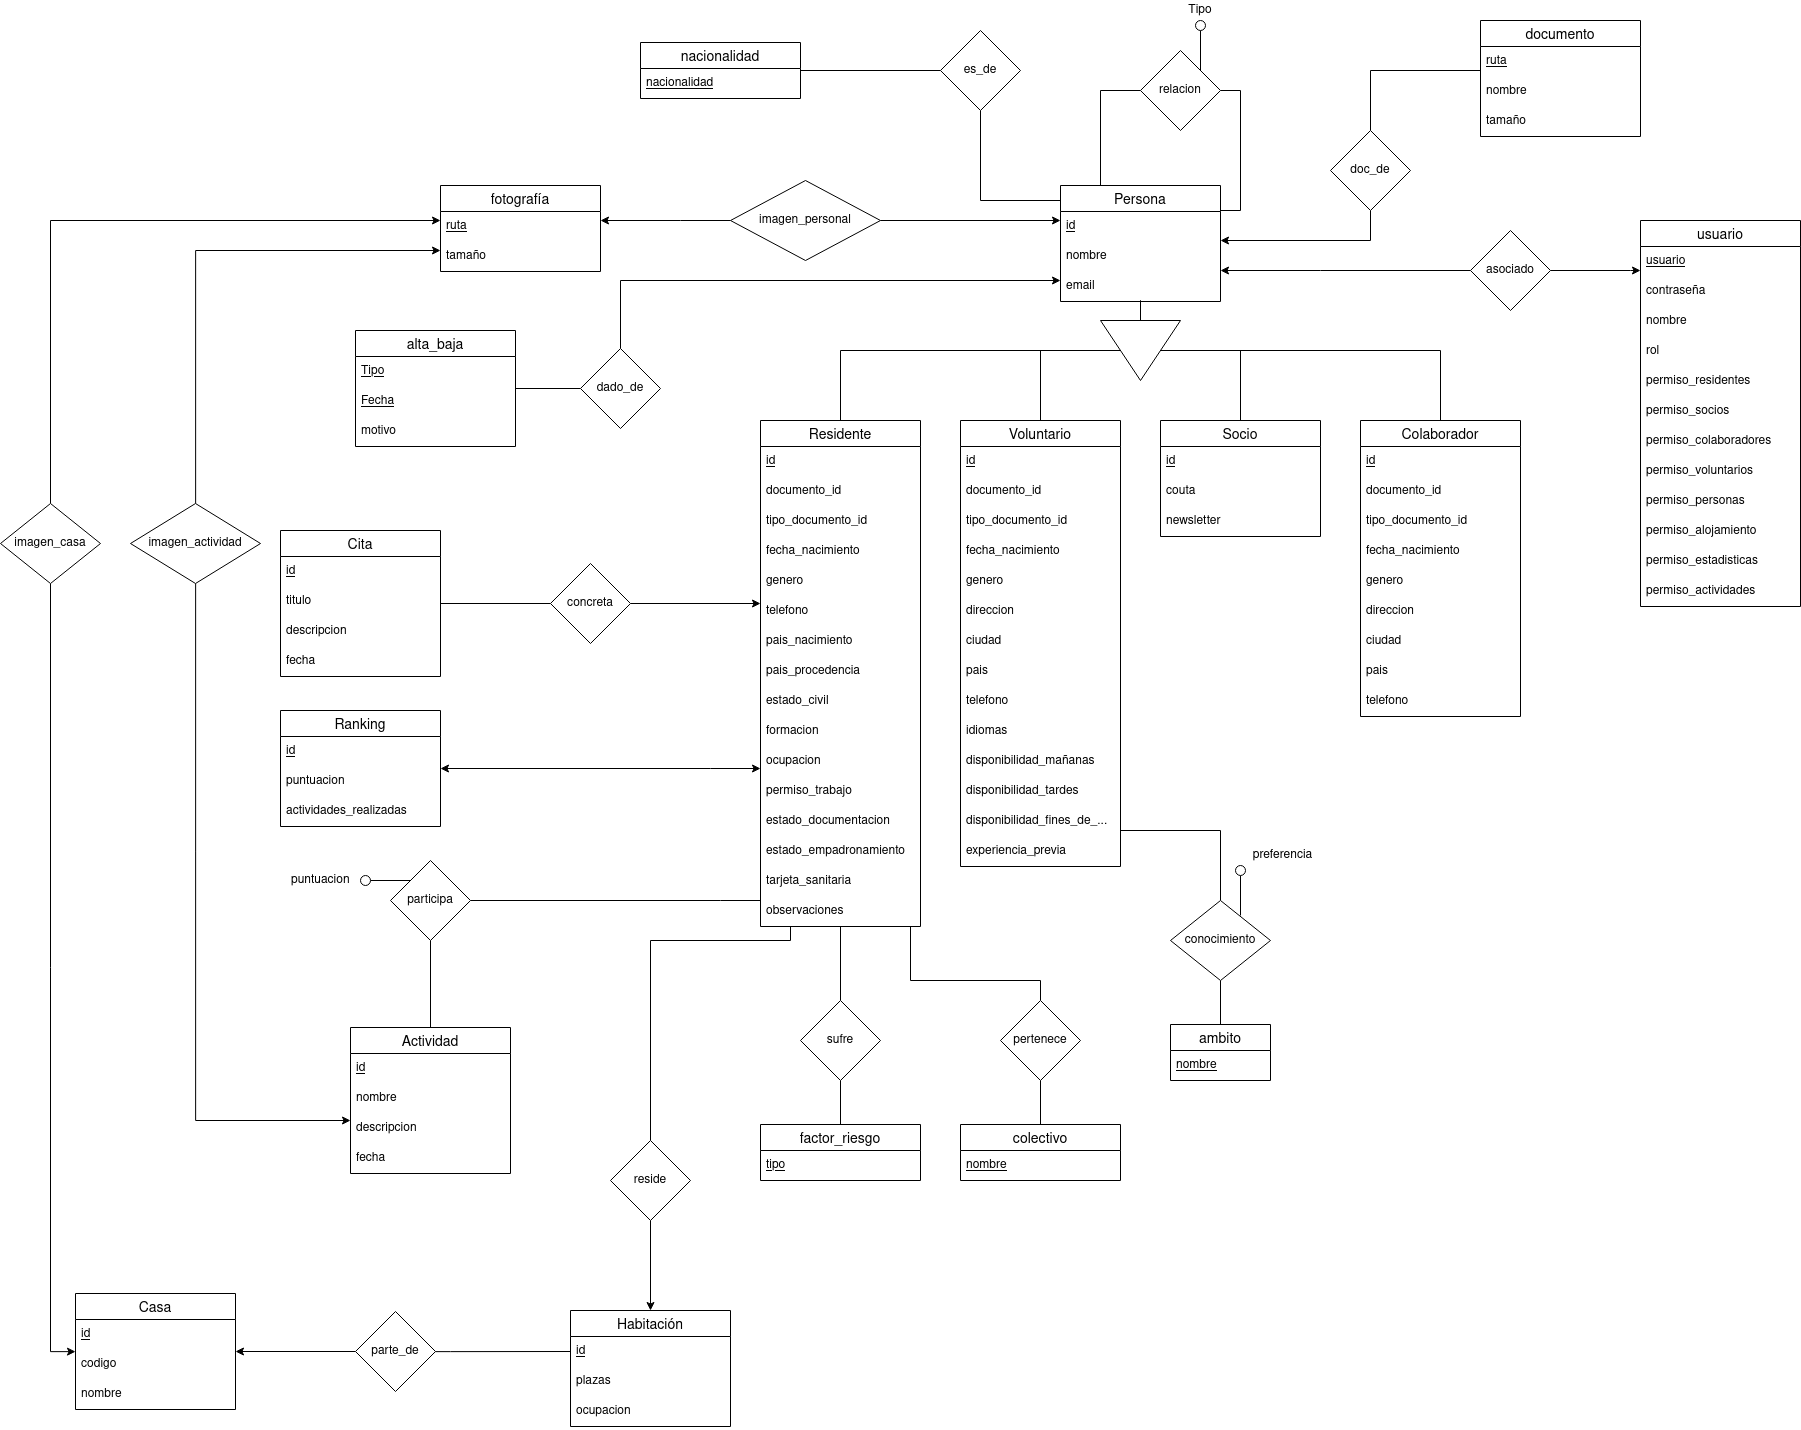
\includegraphics[width=\textwidth]{diseno/base_de_datos/ER.png}
    \caption{Diagrama E/R de la base de datos}
    \label{fig:er}
\end{figure}

\subsection{Diagrama de clases conceptual}

Aunque el desarrollo no siga el paradigma de Programación Orientada a Objetos, con objetivo de aclarar como se comunican los modelos de datos en el sistema, como están relacionados, y que acciones se realizan sobre ellos se ha realizado un diagrama de clases conceptual (Figura \ref{fig:dc}). 

En este se puede destacar la relación de agregación que se produce entre los residentes y las habitaciones, ya que una habitación se compone por residentes, pero entendiéndose que pueda existir una habitación sin residentes. Sin embargo, la relación entre habitación y casa se entiende como una composición, en la que una casa está formada por habitaciones, pero esta no se comprende si no existen habitaciones asociadas.

\begin{figure}[]
    \centering
    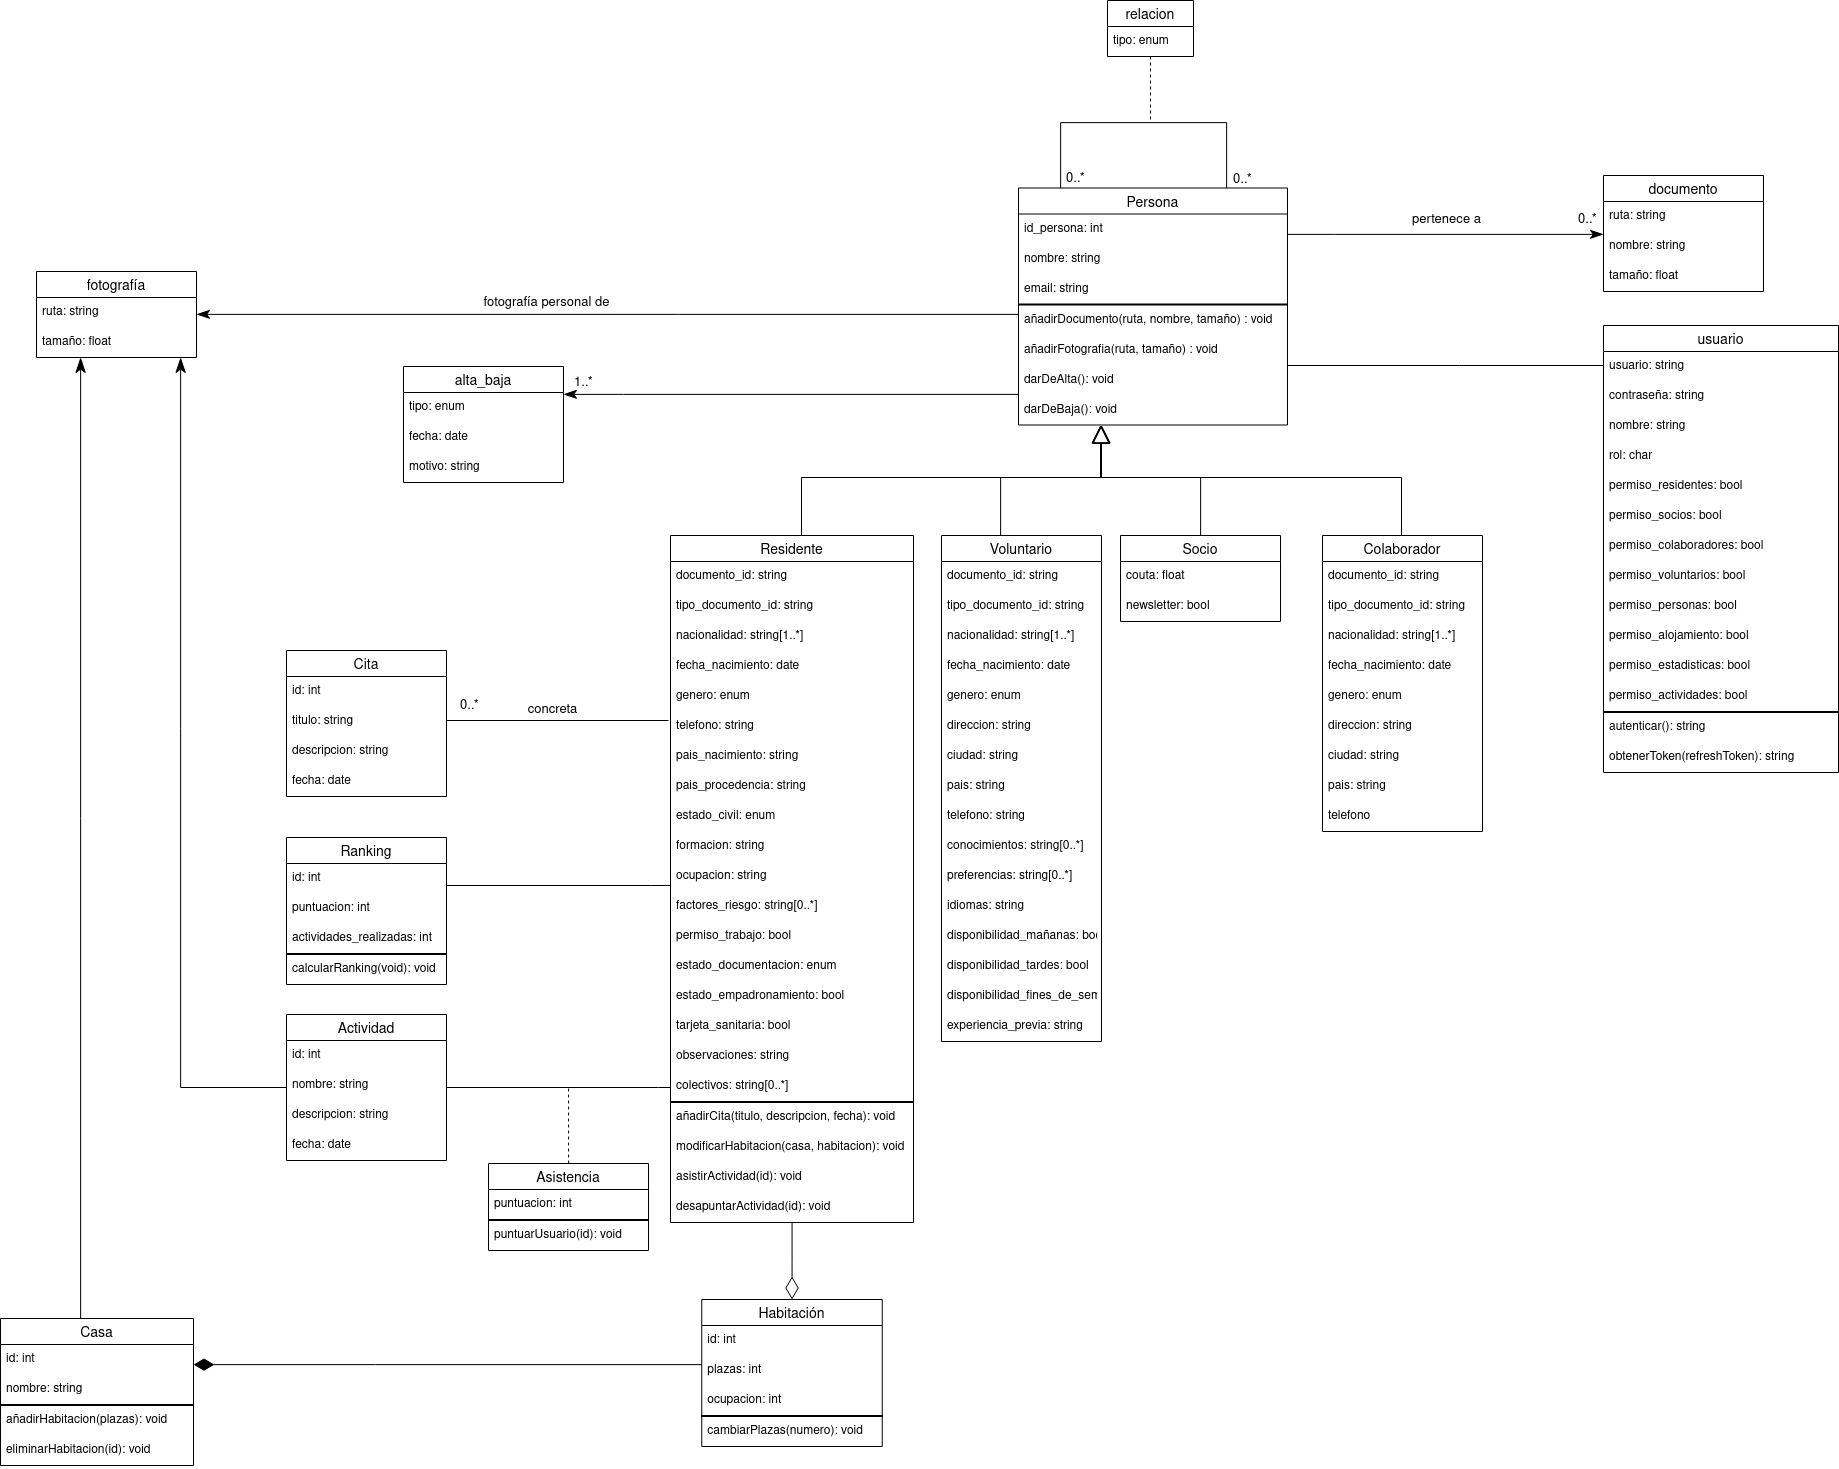
\includegraphics[width=\textwidth]{diseno/sistema/DiagramaDeClases.png}
    \caption{Diagrama de clases conceptual}
    \label{fig:dc}
\end{figure}

